\part{Algorithm} \label{part:algorithm}
% Define the structuring auto-encoder.

\chapter{Background} \label{chap:background}
% Motivation.
% Why ? Neural nets, deep learning, unsupervised feature extraction, representation learning.
% The Need for Non-Local Generalization and Distributed Representations
% Feature learning, representation learning.

\section{Representation learning}
%\section{Feature / representation learning}
% NN is well suited for representation learning
% We want unsupervised feature learning vs supervised vs hand-crafted
% Representation learning
% Learning Distributed Representations: Bengio learning deep ai

\section{Neural networks}
% Why ? Distributed representation and computation (e.g. training on GPU, clusters) --> much what symbolic AI is not (mainly search algorithms, SAT solvers)
% Started in the late 1950s with the perceptron.

\gls{ANNs} are a family of statistical learning models inspired by biological neural networks and are used to estimate or approximate functions that can depend on a large number of inputs and are generally unknown. It is presented as a network of interconnected neurons whose connections have numeric weights that can be tuned based on experience. It makes the neural nets adaptive to inputs and capable of learning.

% What is it ? In general.
Such a network is composed by an input layer, a number of hidden layers and an output layer. The activation of the neurons in the input layer corresponds to the input vector, e.g. an image for computer vision, a song for \gls{MIR}, a word vector for machine translation and sentiment analysis. A weight matrix, followed by a non-linear activation function, then transforms the vector in another representation. The output vector of the first layer is the input vector of the second, and so on until the output layer is reached. The activation of the neurons in the output layer may represent classes, probability distributions, or the estimated value of an unknown function to be learned.

{\color{red} Picture ?}

% Types: feed-forward or recurrent
In a feed-forward network, the connections go from one layer to the next, i.e. information only goes in one direction, forward, from the input nodes, through the hidden nodes (if any) and to the output nodes. Such networks are known to be able to approximate any function. The perceptron, the \gls{MLP} and the \gls{CNN} are examples of this class of networks.
By introducing backward connections, i.e. the connections between units form a directed cycle, we obtain a so called \gls{RNN}. This creates an internal state of the network which allows it to exhibit dynamic temporal behavior. Unlike feed-forward neural networks, an \gls{RNN} can use its internal memory to process arbitrary sequences of inputs. It is known to be able to approximate any program. Such networks have proven very successful for machine translation.

% How to train, supervised.
In a supervised learning setting, the network is trained by back-propagating the error, gradient based learning method, from the output layer to the input through all the hidden layers.
The vanishing gradient problem, where errors shrink exponentially with the number of layers as they propagate from layer to layer, is a major issue of the algorithm \cite{hochreiter2001vanishingGradient}. Various methods, like unsupervised pre-training or \gls{LSTM} \cite{hochreiter1997LSTM}, were developed to work around this problem.

% How to train, unsupervised.
However, in an unsupervised learning setting, there is no desired output, which implies that there is no error to back-propagate. The training algorithm should thus optimize for another objective, which represent desired properties about the output. We will introduce next such an algorithm, called an auto-encoder.

\section{Auto-encoders} \label{sec:auto_encoders}
% For unsupervised learning, i.e. feature extraction.
% Auto-encoders as a manifold learning tool (Bengio review).

An auto-encoder, auto-associator or Diabolo network is an artificial neural network composed of $n$ input and output units and $m$ hidden units. It is used for learning efficient codings \cite{bourlard1988autoencoder, hinton1994autoencoder}. The aim of an auto-encoder is to learn a distributed representation (encoding) for a set of data. An auto-encoder is trained to encode the input $\x \in \R^n$ into some representation $\z \in \R^m$ so that the input can be reconstructed from that representation. It is thus a generative model. Hence the target output of the auto-encoder is the auto-encoder input itself. Auto-encoders may further be stacked to form a \gls{DBN}, while each layer can be trained separately \cite{bengio2007DBN, ranzato2007stackedSparseAutoencoders}.
% Stacked Auto-Encoders, not DBN

{\color{red} Picture ?}

% if linear activations are used, or only a single sigmoid hidden layer, then the optimal solution to an auto-encoder is strongly related to principal component analysis (PCA).[5]
If there is one linear hidden layer and the mean squared error criterion is used to train the network, then the $k$ hidden units learn to project the input in the span of the first $k$ principal components of the data \cite{bourlard1988autoencoder}. If the hidden layer is non-linear, the auto-encoder behaves differently from \gls{PCA}, with the ability to capture multi-modal aspects of the input distribution \cite{japkowicz2000autoencoderPCA}.

The hope is that the code $\z$ is a distributed representation that captures the main factors of variation in the data: because $\z$ is viewed as a lossy representation of $\x$, it cannot be a good representation (with small loss) for all $\x$. So learning drives it to be one that is a good representation in particular for training examples, and hopefully for others as well (and that is the sense in which an auto-encoder generalizes), but not for arbitrary inputs.

It can typically be used for dimensionality reduction by learning a compressed ($m<n$) representation of the data. Another application is feature extraction before classification, for which we want an higher dimensionality ($m>n$) for easier separability. One serious issue with this approach is that if there is no other constraint, then an auto-encoder with $n$-dimensional input and an encoding of dimension $m \geq n$ could potentially just learn the identity function. There are different ways that an auto-encoder with more hidden units than inputs could be prevented from learning the identity, and still capture something useful about the input in its hidden representation $\z$.

\paragraph{Sparse auto-encoders.}
Another strategy, based on the concept of sparse coding, is to add a sparsity constraint on the code. While an ordinary auto-encoder or an \gls{RBM} has an encoder part which computes $P(\z|\x)$ and a decoder part which computes $P(\x|\z)$, sparse coding systems only parametrize the decoder: the encoder is implicitly defined as the solution of an optimization. A middle ground between ordinary auto-encoders and sparse coding was proposed in \cite{lecun2006sparseAutoencoders, ranzato2007stackedSparseAutoencoders} and applied to pattern recognition and machine vision tasks. They propose to let the codes $\z$ be free (as in sparse coding algorithms), but include a parametric encoder (as in an ordinary auto-encoder or \gls{RBM}) and a penalty for the difference between the free non-parametric codes $\z$ and the outputs of the parametric encoder. In this way, the optimized codes $\z$ try to satisfy two objectives: reconstruct well the input (like in sparse coding), while not being too far from the output of the encoder (which is stable by construction, because of the simple parametrization of the encoder). See \secref{encoder} for the definition of our encoder.

\paragraph{Denoising auto-encoders.}
One strategy is to add noise in the encoding. The denoising auto-encoder thus minimizes the error in reconstructing the input from a stochastically corrupted transformation of the input \cite{bengio2008denoisingAutoencoders}. Intuitively, a denoising auto-encoder does two things: try to encode the input (preserve the information about the input), and try to undo the effect of a corruption process stochastically applied to the input of the auto-encoder. This is essentially what a \gls{RBM} does \cite{hinton2002RBM}.


%%%%%%%%%%%%%%%%%%%%%%%%%%%%%%%%%%%%%%%%%%%%%%%%%%%%%%%%%%%%%%%%%%%%%%%%%%%%%%%


\chapter{Model} \label{chap:model}
% Step by step construction: sparse coding, dictionary learning, encoder learning, manifold learning.
% Xavier: maybe not useful as it is just the enumeration of the sub-titles of chapter 2 --> give instead a global motivation.

% Plan.
This chapter presents the proposed structured auto-encoder. \secref{assumptions} states the assumptions of the model. \secref{linear_regression} reviews the basics of linear regression, the foundation of our model. \secref{sparse_coding} introduces sparse coding, \secref{dictionary_learning} introduces a trainable dictionary and \secref{manifold_learning} introduces manifold learning. Last but not least, \secref{encoder} introduces the trainable encoder. Finally, \secref{energy_formulation} reviews the whole energy-based formulation and brings some new insights.

\section{Assumptions} \label{sec:assumptions}
% Xavier: needs to be improved.

\paragraph{Sparse representation.}
We make the hypothesis that a set of sample signals drawn from the same distribution can be sparsely represented in some frame\footnote{A frame of a vector space is a set of vectors which may be linearly dependent. It is a generalization of a basis.}. Each signal should be approximately reconstructed by a linear combinations of a few atoms from a suitable dictionary. As we shall see, this dictionary may be adaptive and learned directly from the data. Many approaches have been developed to achieve sparse representations, e.g. sparse \gls{PCA} \cite{aspremont2007sparsePCA}, sparse NMF \cite{hoyer2004sparseNMF}. Sparse coding \cite{olshausen1996SparseV1, mairal2008sparseCoding} is however the most popular one. Sparsity has become a concept of great interest recently, not only in machine learning but also in statistics and signal processing, in particular with the work on \gls{CS} \cite{candes2005CS, donoho2006CS}.
% There is a huge body of literature on sparse coding and compressed sensing to support this hypothesis.
% --> sparse coding.

% Structured: adding similarity information between inputs.
% Manifold: not all possible signals are reasonable / feasible.
% Xavier: a definition of auto-encoder should be given before in the report.
% We further assume that the subspace spanned by the data is much smaller than the Euclidean space.
\paragraph{Structured data.}
Our second hypothesis is that the dataset holds some structure, in the sense that related samples are close to each other (with respect to some metric). Given a large enough training set, the structure of the data distribution should be able to be captured; i.e. a new valid sample (e.g. from the testing set) should be close to the seen examples.
It suggests that the data is drawn from sampling a probability distribution that has support on or near to a submanifold of the ambient space.
% It suggests that the data lie on a lower dimensional manifold embedded in a high dimensional vector space.
This manifold is however often unknown and must be learned. \gls{SOM} \cite{kohonen1982SOM}, \gls{LLE} \cite{roweis2000LLE}, Laplacian Eigenmaps \cite{belkin2001laplacianEigenmaps} and ISOMAP \cite{tenenbaum2000isomap} are some popular techniques which learn manifolds in a \gls{NLDR} framework. All these algorithms use the so-called locally invariant idea \cite{lecun2006invariantMapping}, i.e. the nearby points are likely to have similar embeddings. Auto-encoders used for dimensionality reduction are able to learn a map from high to low-dimensional space with fewer hidden units than inputs. They are trained to learn to optimally encode the input vectors into a small number of dimensions and decode them back into the original space with minimal error \cite{bourlard1988autoencoder}.
% --> manifold learning.

\paragraph{Encoder.}
We further make the assumption that a simple encoder can be trained to avoid the need of an optimization process that extracts the features during testing, i.e. after the training phase. The encoder shall be more efficient than the optimization process while not degrading too much the quality of the extracted features. Note that even if this hypothesis is not verified, the algorithm is still an auto-encoder, although with an implicit encoder.
% --> auto-encoder.

\section{Linear regression} \label{sec:linear_regression}

\paragraph{Model.}
Given a set $\set{\x}{N} \in \R^n$ of $N$ signals, the subspace $\Xx = \spanning \{\x_i\}_{i=1}^N \subset \R^n$ is defined as the subspace spanned by the data. Then, given a signal $\x \in \Xx$ and a frame $\D \in \R^{n \times m}$, we want to find a representation $\z \in \R^m$ which satisfies the linear regression model
\begin{equation} \label{eqn:linear_regression}
	\x = \D \z + \eps,
\end{equation}
where $\mathbf{\epsilon} \in \R^n$ is the reconstruction error, which is not negligible as long as the frame $\D$ is not complete on $\Xx$.

\paragraph{Capacity.} The hyper-parameter $m$ defines the learning capacity of the auto-encoder. A capacity $m < n$ is good for dimensionality reduction as it exploits the statistical regularities present in the training set while being more compact. A capacity $m > n$ is good for classification as it allows for an easier (linear) separability enabled by the higher dimensional space.

\begin{figure}[ht]
	\centering
	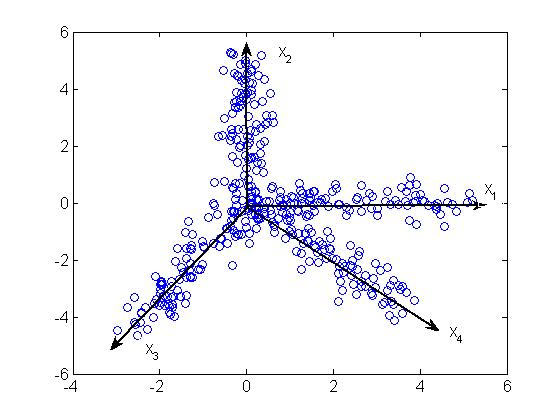
\includegraphics[height=6cm]{img/overcomplete_frame}
	\caption[]{An example of overcomplete frame. While the data lies in a two-dimensional space, a four-dimensional space supported by an overcomplete frame allows a better representation.\footnotemark}
	\label{fig:overcomplete_frame}
\end{figure}
\footnotetext{Figure from Wikipedia.}

\paragraph{Completeness.}
A frame is complete if it can represent any vector $\x \in \Xx$. It is overcomplete if the removal of a vector from the frame results in a complete frame. A set of $n < m$ linearly independent vectors would indeed be overcomplete on the whole space $\R^n$ and a set of $m=n$ linearly independent vectors, like the Fourier transform, would form a basis\footnote{A basis is a set of linearly independent vectors who span the entire space, i.e. it is a linearly independent spanning set.} of $\R^n$, which is obviously complete.

% Complete.
A complete frame which is not overcomplete allows bidirectional lossless transformations. Such problems are well-posed as there exists a unique solution to \eqnref{linear_regression} with $\eps=0$.

% Not complete.
If the frame is not complete, there exist no solution to \eqnref{linear_regression} with $\eps=0$ as the system is overdetermined. An error measure, like \eqnref{least_square} for the \gls{OLS} method, should instead be minimized.

% Overcomplete.
In different research, such as signal processing and function approximation, overcomplete representations have been advocated because they have greater robustness in the presence of noise, can be sparser, and can have greater flexibility in matching structure in the data. However, because of this redundancy, a signal can have multiple expressions under an overcomplete frame \cite{lewicki2000overcompleteRepresentation}. See \figref{overcomplete_frame} for an example of the flexibility of an overcomplete frame to represent a dataset. As there is then an infinite number of solutions to \eqnref{linear_regression} with $\eps=0$, i.e. the problem is ill-posed, a regularization over $\z$ shall be introduced. Optimization techniques are then used to find the optimal solution which minimizes the sum of the error measure and the regularization term, controlled by an hyper-parameter.

\paragraph{Ordinary least squares.}
The method of least squares is a standard approach in regression analysis to the approximate solution of overdetermined systems. "Least squares" means that the overall solution minimizes the sum of the squares of the errors made in the results of every single equation, i.e. it finds
\begin{equation} \label{eqn:least_square}
	\z^* = \argmin{\z} \normT{\x - \D\z},
\end{equation}
where $\normT{\cdot}$ denotes the squared $\ell_2$, or Euclidean, norm. This problem has the closed-form solution
\begin{equation}
	\z^* = (\D^T\D)^{-1} \D^T \x,
\end{equation}
where $T$ denotes the matrix transpose. The primary assumption of \gls{OLS} is that there are zero or negligible errors in the independent variable $\D$, since this method only attempts to minimize the mean squared error in the dependent variable $\x$. That is not an issue in an auto-encoder setting where $\D$ is either hand-crafted or learned.

% underdetermined == ill-posed ?
\paragraph{Regularization.}
% L2.
Tikhonov regularization \cite{tikhonov1963tikhonovRegularization}, or ridge regression, is the most commonly used method of regularization of ill-posed problems. It adds a prior of the form $\lambda \normT{\gam \z}$ to the minimization problem \eqnref{least_square} as follows:
\begin{equation} \label{eqn:tikhonov_regularization}
	\z^* = \argmin{\z} \normT{\x - \D\z} + \lambda \normT{\gam \z},
\end{equation}
where $\gam$ is the Tikhonov matrix. This matrix is often chosen to be a multiple of the identity matrix, i.e. $\gam = \alpha \mathbf{I}$, giving preference to solutions with smaller norms. In a Bayesian context, this is equivalent to placing a zero-mean normally distributed prior on $\z$ \cite{vogel2002inverseProblems}. In other cases, lowpass operators, e.g. a difference operator or a weighted Fourier operator, may be used to enforce smoothness if the underlying vector is believed to be mostly continuous. A regularization of this kind will be introduced in our model in \secref{manifold_learning}. An explicit solution is given by
\begin{equation}
	\z^* = (\D^T\D + \gam^T\gam)^{-1} \D^T \x.
\end{equation}

% L1.
Another commonly used regularization is the \gls{LASSO} \cite{tibshirani1996Lasso}, which adds the prior $\lambda \normO{\z}$ to the minimization problem \eqnref{least_square} as follows:
\begin{equation} \label{eqn:lasso_regularization}
	\z^* = \argmin{\z} \normT{\x - \D\z} + \lambda \normO{\z},
\end{equation}
where $\normO{\z} = \sum_{i=1}^{m} |z_i|$ is the $\ell_1$ norm of $\z$, also called the Taxicab or Manhattan norm.
In a Bayesian context, this is equivalent to placing a zero-mean Laplace prior distribution on $\z$ \cite{park2008BayesianLasso}. The advantage of the \gls{LASSO} is that it promotes the simplest solutions, i.e. the solutions with many zeros. Driving parameters to zero effectively deselects the features from the regression. \gls{LASSO} thus automatically selects the most relevant features, whereas ridge regression never fully discards any. For this reason, the \gls{LASSO} and its variants are fundamental to the field of \gls{CS}. A regularization of this kind will be introduced in our model in \secref{sparse_coding}.

% L1 + L2.
An extension of this approach is the elastic net regularization \cite{zou2005ElasticNet} which linearly combines the $\ell_1$ and $\ell_2$ penalties of the \gls{LASSO} and ridge methods as follows:
\begin{equation} \label{eqn:elasticnet_regularization}
	\z^* = \argmin{\z} \normT{\x - \D\z} + \lambda_2 \normT{\z} + \lambda_1 \normO{\z}.
\end{equation}
This regularization overcomes some limitations of the $\ell_1$ penalty, e.g. the saturation which happens for high-dimensional data with few examples, or the fact that the \gls{LASSO} tends to select only one variable and ignore the others if there is a group of highly correlated variables.

\section{Sparse coding} \label{sec:sparse_coding}
% What it is, why it works, why it's good.
% paper who demonstrates that L1 penalty leads to same solution as L0 while being convex, not combinatorial

% Sparse coding.
The main idea behind sparse coding \cite{olshausen1996SparseV1, mairal2008sparseCoding} is to express the signal $\x \in \Xx \subset \R^n$ as a sparse linear combination of basis functions $\set{\d}{m} \in \R^n$, or atoms, from an overcomplete dictionary $\D \in \R^{n \times m}$. The sparse code $\z^* \in \R^m$ is given by
\begin{equation} \label{eqn:sparsecoding}
	\z^* = \argmin{\z} \frac{\lambda_d}{2} \normT{\x - \D \z} + \lambda_z \normZ{\z},
\end{equation}
where $\normZ{\z}$ denotes the number of non-zero elements in $\z$.  $\lambda_d$ and $\lambda_z$ are the (redundant) hyper-parameters setting the trade-off between the data term, an accurate reconstruction, and the prior, a sparse solution. Overcomplete sparse representations tend to be good features for classification systems as they provide a succinct representation of the signal, are robust to noise and are more likely to be linearly separable due to their high dimensionality.

% Faster sparse coding approximations.
Finding the sparse code $\z^*$ however requires a combinatorial search which is an NP-hard problem \cite{natarajan1995sparseNPhard}, intractable in high dimensional spaces. Various approximations have thus been proposed. \gls{MP} \cite{mallat1993MatchingPursuit} offers a greedy approximation to the solution while \gls{BP} \cite{chen1998BasisPursuit} is the popular convex approximation
\begin{equation} \label{eqn:basispursuit}
	\z^* = \argmin{\z} \frac{\lambda_d}{2} \normT{\x - \D \z} + \lambda_z \normO{\z},
\end{equation}
which is the \gls{LASSO} regularized least square problem introduced in \eqnref{lasso_regularization}. As is now well understood \cite{candes2005CS, donoho2006CS}, the $\ell_1$ norm is a very good proxy for the $\ell_0$ pseudo-norm and naturally induces sparse results. It can even be shown to recover exactly the true sparse code, i.e. the solution of \eqnref{sparsecoding} (if there is one), under mild conditions \cite{donoho2003OptSparse}. {\color{red}link with \gls{RIP}}. A number of algorithms have been proposed to efficiently solve this problem \cite{chen1998BasisPursuit, beck2009FISTA, ng2006EfficientSparse, li2009Coordinate}. They however still rely on computationally expensive iterative procedures which limit the system's scalability and real-time applications. While a direct method will always be preferred for feature extraction, iterative methods will still be necessary during training. Distributed computing with \gls{GPU} or via cloud computing will hopefully accelerate the process.

\section{Dictionary learning} \label{sec:dictionary_learning}

% Why ?
\paragraph{Model.}
In classical sparse coding, the dictionary is composed of known functions such as sinusoids \cite{bracewell1965fourier}, wavelets \cite{mallat1999wavelet}, Gabors \cite{gabor1946gabor}, curvelets \cite{candes2002curvelet} or contourlets \cite{vetterli2003contourlet}; i.e. hand-crafted features. One may also want to learn a dictionary that is adaptive to the type of data at hand. This approach may allow an even more compact representation and may lead to the discovery of previously unknown discriminative features.
% gammatones\footnote{A gammatone is a sinusoid (a pure tone) with an amplitude envelope which is a scaled gamma distribution function. It is used to build cochlear models.} \cite{holdsworth1992gammatone}

% How ?
To use the dictionary $\D$ as an unknown variable, all the training data shall be part of the objective function as the dictionary depends on all of them. The energy function, composed by an $\ell_2$ fidelity term and an $\ell_1$ penalty, becomes
\begin{equation} \label{eqn:en_dict}
	\Eone = \frac{\lambda_d}{2} \normF{\X - \D \Z} + \lambda_z \normO{\Z},
\end{equation}
where $\normF{\cdot}$ denotes the squared Frobenius norm, $\X = \set{\x}{N} \in \R^{n \times N}$ is the set of training vectors and $\Z = \set{\z}{N} \in \R^{m \times N}$ their associated sparse codes. $N$ is naturally the number of training vectors, which should be much greater than the size $m$ of the dictionary to avoid the trivial solution where examples are copied in the dictionary. The problem to solve is then
\begin{equation} \label{eqn:pr_dict}
	\minimize{\Z,\D} \Eone \st \cstd,
\end{equation}
where the $\ell_2$ ball constraint (usually implemented by rescaling the columns $\d_i$ of $\D$ at each iteration) prevents the trivial solution where the code coefficients go to zero while the bases are scaled up. While this problem is not convex, a good approximate solution can be found by iteratively minimizing for $\Z$ and $\D$ \cite{olshausen1996SparseV1}.
% Simple gradient descent or more sophisticated methods \cite{chen1998BasisPursuit, beck2009FISTA, li2009Coordinate} for $\z$, stochastic gradient descent for $\D$.

\paragraph{Completeness.}
The learned dictionary may be seen as an overcomplete frame of the subspace $\Xx$ spanned by the training data. The overcompleteness of the learned dictionary could indeed be tested: the frame should be able to perfectly represent any training sample, i.e. in the absence of the $\ell_1$ regularization, the reconstruction error $\eps$ of \eqnref{linear_regression} should be zero.

% Motivation: learned dictionaries resemble brain processing stages.
\paragraph{Biological motivation.}
There is evidence that sparse coding may be a strategy employed by the brain in the early stages of visual and auditory processing \cite{olshausen1996SparseV1, olshausen1997SparseV1, smith2006SparseAudio}. Basis functions learned on natural images have been shown to resemble the receptive fields of neurons in the visual cortex \cite{olshausen1996SparseV1, olshausen1997SparseV1}. Basis functions learned on natural sounds were found to be highly similar to gammatone functions \cite{smith2006SparseAudio} which have been used to model the action of the basilar membrane in the inner ear. Moreover, learning on natural time-varying stimuli such as speech or video has been shown to produce localized bases \cite{lewicki2000SparseSpeech, olshausen2000SparseVideo}.

\section{Manifold learning} \label{sec:manifold_learning}
% Further structure, geometry learning.
% Three parts: manifold, graph and model.

% Why ?
\paragraph{Motivation.}
% Paper: graph regularized sparse coding.
Most of the existing approaches to sparse coding fail to consider the geometrical structure of the data space. The data is however more likely to reside on a low-dimensional submanifold embedded in the high-dimensional ambient space.
%It has been shown that the geometrical information of the data is important for discrimination \cite{zheng2011StructuredSparse}.
It has been shown that learning performance can be significantly enhanced if the geometrical structure is exploited and the local invariance is considered  \cite{zheng2011StructuredSparse}.

% General introduction.
%\paragraph{Manifold.}
%A manifold is a topological space that resembles Euclidean space near each point, i.e. each point of an $d$-dimensional manifold has a neighborhood that is homeomorphic to the Euclidean space of dimension $d$. Lines and circles, but not figure eights, are one-dimensional manifolds. Two-dimensional manifolds are also called surfaces. Examples include the plane, the sphere, and the torus, which can all be embedded in three-dimensional real space. \figref{manifolds} shows examples of 1D and 2D manifolds.

%\begin{figure}[ht]
%	\centering
%	\begin{subfigure}[b]{0.49\textwidth}
%		\centering
%		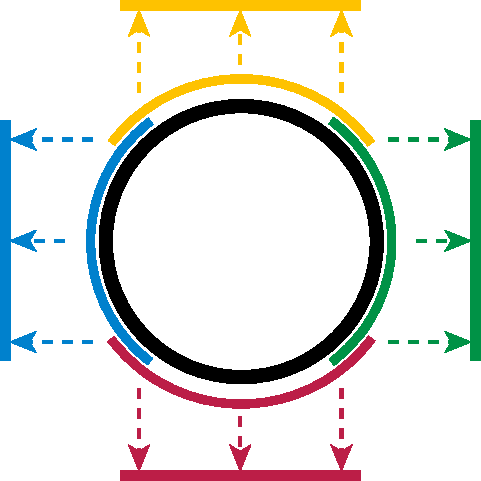
\includegraphics[height=6cm]{img/circle_manifold_charts}
%		\caption{}
%	\end{subfigure}
%	\begin{subfigure}[b]{0.49\textwidth}
%		\centering
%		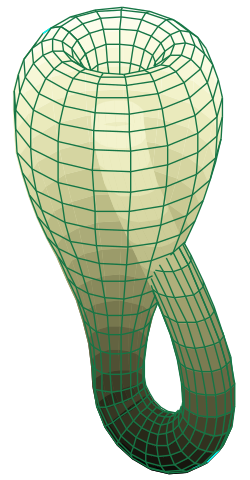
\includegraphics[height=6cm]{img/klein_bottle}
%		\caption{}
%	\end{subfigure}
%	\caption[]{Examples of manifolds.\footnotemark (a) The circle, a 1D manifold, can be mapped by four charts. (b) The klein bottle is a 2D manifold that cannot be embedded in a 3D space without self-intersection.}
%	\label{fig:manifolds}
%\end{figure}
%\footnotetext{Figures from Wikipedia.}

% Example close to our case.
%Let's imagine a single handwritten digit recognition system. The input is an image of $n \times n$ pixels which is represented by a vector $\x \in \R^{n \times n}$. However, not all vectors $\x \in \R^{n \times n}$ represent meaningful data. The vast majority indeed represents garbage. We may make the hypothesis that the set of plausible digits lies on a $d$-dimensional manifold where $d \leq n \times n$.

% Approximate a manifold.
%The problem is that we often ignore the shape of the embedded manifold. We only have at our disposal some samples which are drawn from it, e.g. a few examples of handwritten digits. Another example with object scanning: we obtain a discrete point cloud sampled from the surface. We do know some points on the surface, but we don't know the exact surface.

%We use graphs as discrete approximations of low-dimensional manifolds embedded in high-dimensional spaces. The set of data are samples drawn from this unknown manifold.

% General formulation.
% What a graph is, generally. Not only a manifold approximation.
\paragraph{Similarity graphs.}
% Paper: Pierre's review
Graphs are generic data representation forms which are useful for describing the geometric structures of data domains in numerous applications, including social, energy, transportation, sensor, and neuronal networks \cite{pierre2013graphs}. The connectivity and weight associated with each edge in the graph is either dictated by the physics of the problem at hand or inferred from the data.
Weighted graphs are commonly used to represent similarities between data points in statistical learning problems for applications such as machine vision \cite{lowe1999graphSimilarity} and automatic text classification \cite{apte1994graphSimilarity}.

%\begin{figure}[ht]
%	\centering
%	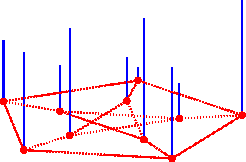
\includegraphics[height=6cm]{img/example_graph}
%	\caption[]{A random positive graph signal on the vertices of the Petersen graph. The height of each blue bar represents the signal value at the vertex where the bar originates.\footnotemark}
%	\label{fig:example_graph}
%\end{figure}
%\footnotetext{Figure from \cite{pierre2013graphs}.}

% We first review some basic definitions and notations from spectral graph theory and then show how we can use a graph to approximate a manifold.

% Graph definition.
From the set of training vectors $\X$, we can construct an undirected, connected and weighted graph $\G = \{ \V, \varepsilon, \W \}$ which consists of a finite set of vertices $\V$ with $|\V| = N$, a set of edges $\varepsilon$, and a weighted adjacency matrix $\W = (w_{ij}) \in \R^{N \times N}$. Each vertex $i \in \V$ represents a training vector $\x_i$. If there is an edge $e = (i, j)$ connecting vertices $i$ and $j$, the entry $w_{ij}$ represents the weight of the edge; otherwise, $w_{ij} = 0$. The set of sparse codes $\Z$ is a signal which resides on the graph, i.e. a signal with one sample $\z_i$ at each vertex $i$ of the graph.

% Distance metric: euclidean (small dim) and cosine (angular, high dim).
% ref for why cosine is better in high dim
% Intuition: cosine is euclidean when data projected to sphere.
% Kernel: Gaussian or polynomial.
While their exists several ways to define the edge weights when they are not naturally defined by the application, they often represent the similarity between the two vertices they connect \cite{pierre2013graphs}. For instance, the edge weight may be inversely proportional to the Euclidean distance between the vectors:
\begin{equation}
	w_{ij} = \exp \left( - \frac{\normT{\x_i - \x_j}}{2\sigma^2} \right) \in [0,1],
\end{equation}
where the Gaussian kernel width $\sigma$ controls the width of the neighborhoods and $\inner{\cdot}{\cdot}$ denotes the scalar product. While the Euclidean distance is a good choice for low-dimensional data, its discriminative power vanishes in higher dimensional space {\color{red} [ref?]}. An option is then to use the cosine similarity as the edge weight:
\begin{equation}
	w_{ij} = \frac{1}{2} + \frac{1}{2} \cos(\theta) = \frac{1}{2} \left(1 + \frac{\inner{\x_i}{\x_j}}{\|\x_i\|_2 \|\x_j\|_2} \right) \in [0,1],
\end{equation}
where $\theta$ is the angle between the two vectors $\x_i$ and $\x_j$. Another reason for the popularity of the cosine similarity is that it is very efficient to evaluate, especially for sparse vectors, as only the non-zero dimensions need to be considered. See \cite{grady2010graphs} for other graph
construction methods.

% Type: KNN vs epsilon.
A fully connected graph is usually not wanted: the number of edges are often artificially limited in order to reduce the storage and computational cost associated with the graph manipulation, effectively sparsifying the weight matrix $\W$.
The $\epsilon$-neighborhood graph is the popular approach which sets to 0 any weigh $\W_{i,j} < \epsilon$ for some threshold $\epsilon$. While being useful for mathematical derivations, this approach is unstable when the data is not uniformly sampled.
A second common method is to connect each vertex to its $k$-nearest neighbors only and drop the smallest weights; in which case \cite{zelnik2004scale} suggests to set the Gaussian kernel scale $\sigma$ to the mean of the $k^{\text{st}}$ distances.

\paragraph{Graph Laplacian.}
% The graph (normalized) Laplacian is an approximation of the Laplace-Beltrami operator. --> Dirichlet energy
% normalized vs un-normalized, cite normalized approximates the Laplace-Beltrami operator
% A way to test if the Laplacian is well constructed is... (see blog)
% Another regularization on Z. Like Thikonov with the graph Laplacian as the Tikhonov matrix (difference operator). It enforces smoothness on the graph / manifold.
% The graph Laplacian as a difference operator.
% \L = U \Lambda U^*, U Fourier basis, Lamb eigenvalues / frequencies, U* inverse Fourier.
The unnormalized graph Laplacian, also called the combinatorial graph Laplacian, is defined as
\begin{equation}
	\L = \A - \W,
\end{equation}
where the degree matrix $\A=(a_{ij}) \in \R^{N \times N}$ is a diagonal matrix whose $i$th diagonal element $a_{ii}$ is equal to the sum of the weights of all the edges incident to vertex $i$:
\begin{equation}
	a_{ii} = \sum\limits_{j=1}^{N} w_{ij}.
\end{equation}
The graph Laplacian is a difference operator as it satisfies
\begin{equation}
	\L\z_i = \sum\limits_{j=1}^{N} w_{ij} (\z_i - \z_j).
\end{equation}

\paragraph{Dirichlet energy.}
The Dirichlet energy is a measure of the smoothness of a graph signal given by
\begin{equation} \label{eqn:dirichlet_energy}
	\tr(\Z\L\Z^T) = \frac{1}{2} \sum\limits_{i=1}^{N} \sum\limits_{j=1}^{N} w_{ij} \normT{\z_i - \z_j} \geq 0,
\end{equation}
which is a suitable candidate for regularization \cite{belkin2006manifoldRegularization}.
%\paragraph{Manifold assumption.}
The assumption that the representations $\Z$ should be smooth on the similarity graph $\G$ constructed by the training vectors $\X$, usually referred to as the manifold assumption, plays an essential role in various kinds of algorithms including dimensionality reduction algorithms \cite{belkin2001laplacianEigenmaps}, clustering algorithms \cite{ng2002spectralClustering} and semi-supervised learning algorithms \cite{belkin2006manifoldRegularization, zhou2004manifoldRegularization}.
% exploit the geometrical information in the data by using the manifold assumption which has been shown effective in classification and clustering tasks \cite{belkin2006manifoldRegularization}.

% Why normalized Laplacian ? Consistency.
% Descrete graph Laplacian converges to continuous Laplace-Beltrami operator.
% Reference: Erdos.
% Why graphs ? To approximate the unknown manifold.
% Correct approximation because of the consistency principle.
% While the dataset $\X$ is supposedly drawn from a manifold, the manifold itself is unknown.
\paragraph{Consistency.}
Two normalized graph Laplacians are found in the literature \cite{chung1997spectralGraphTheory}:
\begin{equation}
	\L_{sym} = \A^{-1/2} \L \A^{-1/2} = \I - \A^{-1/2} \W \A^{-1/2},
\end{equation}
and
\begin{equation}
	\L_{rw} = \A^{-1} \L = \I - \A^{-1} \W,
\end{equation}
where $\I$ denotes the identity matrix.
While there is no convergence guarantee for the unnormalized graph Laplacian, these two normalized Laplacian can be shown to converge to the continuous Laplace-Beltrami operator as the number of samples increase \cite{vonluxburg2008consistency}. The similarity graph is indeed a good approximation of the unknown manifold.

\paragraph{Model.}
% Paper: By using graph Laplacian as a smooth operator, the obtained sparse representations vary smoothly along the geodesics of the data manifold.
The geometrical information about the data is encoded in a similarity graph constructed by the training vectors $\X$ and the graph Laplacian is used as a smooth operator to preserve the local manifold structure. Introducing the Dirichlet energy into the objective function as an additional $\ell_2$ regularization, similar to the Tikhonov regularization presented in \secref{linear_regression}, gives
\begin{equation}\label{eqn:en_structure}
	\Etwo = \frac{\lambda_d}{2} \normF{\X - \D \Z} + \lambda_z \normO{\Z} + \lambda_g \tr(\Z^T \L \Z).
\end{equation}
This regularization promotes a smooth variations of the representations along the geodesics of the data manifold.

\section{Encoder} \label{sec:encoder}
% Auto-encoder: explicit encoder instead of implicit encoder.
% Problem: these methods are slow at inferring sparse codes as they need iterations
% --> train an encoder

\paragraph{Motivation.}
In order to avoid the iterative procedure typically required to infer the sparse code, we aim at an explicit encoder which can quickly map inputs to approximations of their sparse code. Several works \cite{lecun2010PSD, lecun2010LISTA, lecun2013DrSAE} {\color{red} [others not from LeCun?]} have been done in this direction. The addition of an encoder to the sparse coding scheme leads to the sparse variant of auto-encoders which was introduced in \ref{sec:auto_encoders}.

% 2nd motivation.
Moreover, adding structure to the problem should enhance the behavior of the loss function and help sparse recovery \cite{kowalski2009sparse, baraniuk2010modelCS, huang2011LearningStructuredSparsity, jenatton2011structured}. {\color{red}Then \cite{donoho2003OptSparse} should not be strong enough.}

% How ?
\paragraph{Model.}
Introducing a trainable encoder $\E \in \R^{m \times n}$, which should predict sparse codes from input vectors with minimum error, into our model gives the energy function
\begin{equation}\label{eqn:en_encoder}
	\Ethree = \frac{\lambda_d}{2} \normF{\X - \D \Z} + \lambda_z \normO{\Z} + \lambda_g \tr(\Z^T \L \Z) + \frac{\lambda_e}{2} \normF{\Z - \E \X}, %{\color{red} + \lambda_s \normO{\E \X}},
\end{equation}
%where $\lambda_e$ and $\lambda_s$ are two additional hyper-parameters which control the sparsity versus fidelity tradeoff. The problem is then defined by
where $\lambda_e$ is an additional hyper-parameter which controls relative weight of the prediction error. The problem is then defined by
\begin{equation}\label{eqn:pr_encoder}
	\minimize{\Z,\D,\E} \Ethree \st \cst{\d}{i} , \cst{\e}{k} ,
	\ \forallx{i}{m} , \ \forallx{k}{n},
\end{equation}
where $\e_k$ are the columns of $\E$. %Again, the $\ell_1$ penalty $\normO{\E \X}$ regularizes the least square problem, i.e. the \gls{LASSO} method.

\paragraph{Energy.}
While it is often a good idea to control the energy, the constraint on the columns of $\E$ is not needed in practice. While the columns of $\D$ are constrained to a norm smaller than one, they are in practice normalized because of the $\normO{\Z}$ objective. The energy of a vector transformed by $\D$ does thus not change, which means that the inferred sparse code $\z_i$ as the same energy as its corresponding vector $\x_i$. The encoder does then not need to add energy and will have a column norm smaller than one, even without the constraint. It has been verified empirically.

\newpage
\section{Energy-based formulation} \label{sec:energy_formulation}
% energy-based model
% Why energy ?

% Finish with the complete objective function.
% Why energy function ? Many laws of nature are nothing but optimality conditions, often expressed in terms of a minimum energy principle.
% Easy to add and remove terms.
% the sparsity constraint prevents the auto-encoder to learn the identity

{\color{red} Image with input x and hidden z. Output is y=sh(Ex). Weight matrices are D and E with sh() activation function. Approximately.}

% Sparse coding: terms ..
% Auto-encoders: terms ..
% Manifold learning: terms ..
% Regularized least square (elastic net): terms ..

Our overall model may be thought as an hybrid between a sparse and a denoising auto-encoder.

% Identify parts of the energy functions to equations in regression, e.g. tik, lasso, elastic.

%%%%%%%%%%%%%%%%%%%%%%%%%%%%%%%%%%%%%%%%%%%%%%%%%%%%%%%%%%%%%%%%%%%%%%%%%%%%%%%


\chapter{Learning through optimization} \label{chap:learning}
% Learning / Training
% Non-convex problem where each sub-problem / independant variable is a convex problem --> outer loop --> objective monotically decreasing.
% Batch (FISTA, primal-dual) and online (stochastic gradient descent) training
% Transductive learning
% Non-convex problem composed of convex sub-problems.
% Derive prox and gradients.
% Why we can use FISTA an PD ?
% Derive FISTA and primal-dual formulations.

% Only the sub-problems are convex.
Although the objective function in (2) is convex in only
or only, it is not convex in both variables together. A nat-
ural approach to solve this problem is to iteratively optimize the
objective function (2) by minimizing over one variable while
keeping the other one fixed. Thus, it becomes an -regular-
ized least squares problem plus an -constrained least squares
problem, which can both be solved efficiently by several opti-
mization methods.

% An alternative for the dictionary part.
One of the most efficient methods is the K-SVD method [28]. The K-SVD is a way to learn a dictionary, instead of exploiting standard bases as described previously, that leads to sparse representations for the data. This algorithm uses ei- ther orthogonal matching pursuit (OMP) or basis pursuit (BP), as part of its iterative procedure for learning the dictionary.

\section{Convex problem}
% What is a convex problem (objective and constraints).
% Methods to solve: analytically or numerical schemes.

\section{Numerical solvers}
% Numerical: gradient descent --> slow --> second order methods like Newton
% Stochastic gradient descent

\section{Proximal splitting methods}
% But our objective function is not differentiable
% Ridge regression is, but not the LASSO regularization.
% --> rely on a sub-gradient method, the proximity / proximal operator --> proximal splitting

\subsection{Forward-backward}
% Different basic methods to solve these problems: forward-backward, douglas-rachford
% Explain the intuition

\subsection{Douglas-Rachford}

\subsection{FISTA}
% Advanced (faster) algorithms who exlpoit variable time steps and multiple points: FISTA

\section{Dual problem}
% Introducing the dual problem (paper playing with duality)

\subsection{Primal-dual}

%%%%%%%%%%%%%%%%%%%%%%%%%%%%%%%%%%%%%%%%%%%%%%%%%%%%%%%%%%%%%%%%%%%%%%%%%%%%%%%

\chapter{Related work} \label{chap:related_work}
% How do we compare with other auto-encoders ?
% Sparse: Corresponds to 2 of our terms.
% Denoising: The manifold terme pushes the samples back to the manifold, effectively denoising the samples.